\UC{Ricerca dei prodotti} 
L'utente non autenticato o l'acquirente può cercare i prodotti dalla schermata principale oppure dalla PLP.
\begin{itemize}
    \item \textbf{Attori primari:} acquirente o utente non autenticato;
    \item \textbf{Precondizione:} l'attore ha selezionato l'azione della ricerca e inserito le parole per la ricerca del prodotto;
    \item \textbf{Postcondizione:} l'attore viene reindirizzato alla PLP con i prodotti che contengono nella descrizione o nel nome, almeno una delle parole per le quali si è svolta la ricerca;
    \item \textbf{Scenario principale:} l'attore ha selezionato l'azione della ricerca e inserito le parole per la ricerca del prodotto. In seguito preme sull'azione di ricerca e viene reindirizzato alla PLP che contiene tutti i prodotti che hanno almeno una delle parole indicate nella descrizione o nel nome;
    \end{itemize}
    \item \textbf{Estensioni:}
    \begin{enumerate}[label=\lett]
        \item L'attore ha svolto una ricerca che non ha prodotto alcun risultato. In questo caso:
        \begin{itemize}
            \item (UC) - Viene visualizzato il messaggio di ricerca senza alcun risultato.
        \end{itemize}
    \end{enumerate}
\end{itemize}

\UC{Filtraggio prodotti della PLP}
\begin{figure}[H]
    \centering
    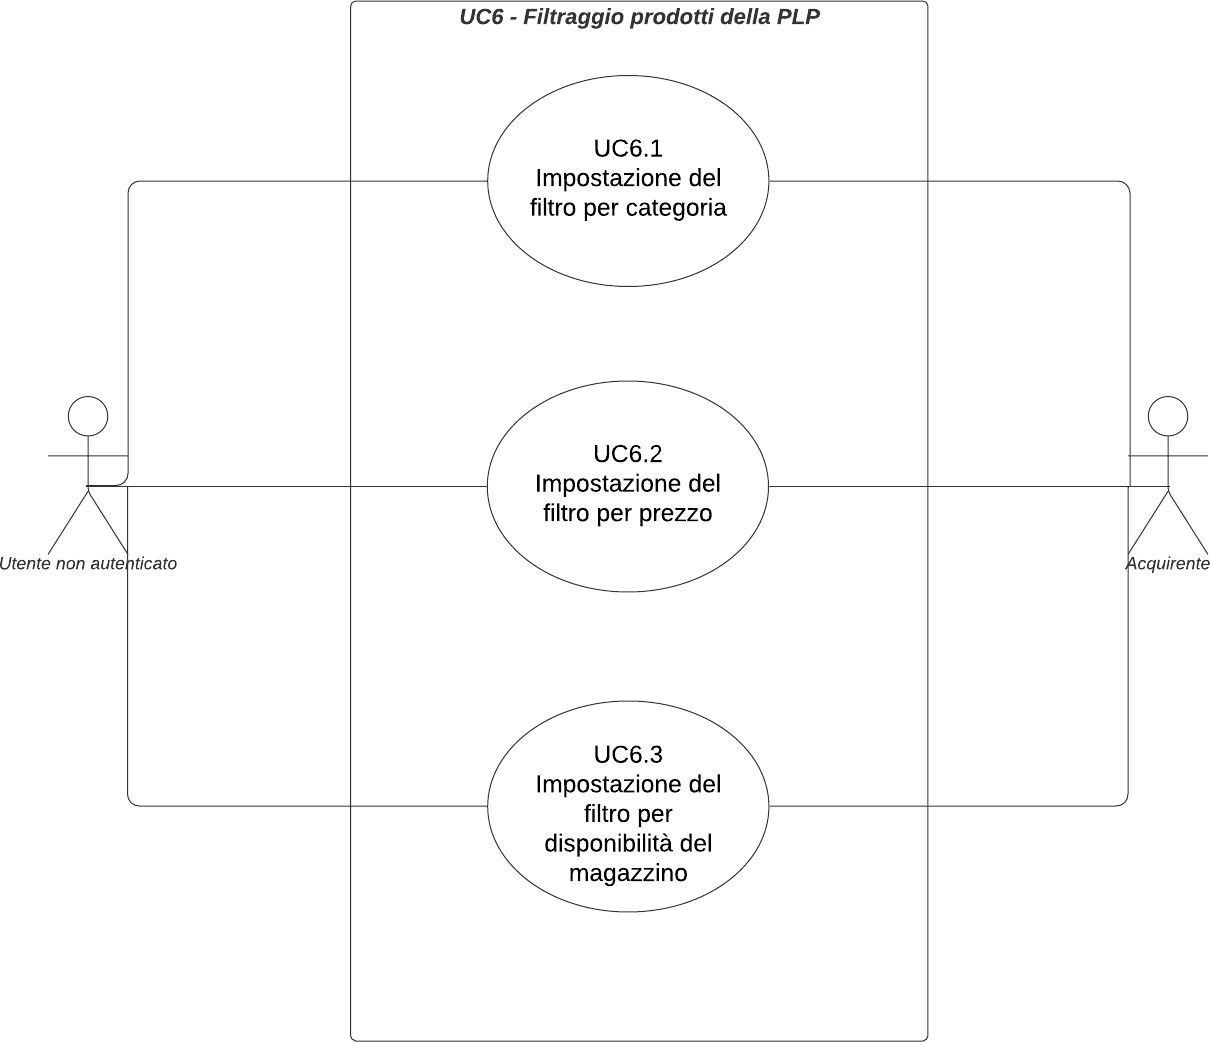
\includegraphics[scale=0.5]{Immagini/DiagrammiUC/UC6FiltraggioProdottiDellaPLP.png}
    \caption{Diagramma di \actualUC: Filtraggio dei prodotti della PLP} 
\end{figure}

L'utente non autenticato o l'acquirente può filtrare i prodotti all'interno della PLP per categoria, prezzo, promozioni attive, sconti applicati e se c'è disponibilità nel magazzino.
\begin{itemize}
    \item \textbf{Attori primari:} acquirente o utente non autenticato;
    \item \textbf{Precondizione:} l'attore è nella PLP e ha impostato uno (o più) dei filtri disponibili per i quali cercare;
    \item \textbf{Postcondizione:} l'attore avrà a disposizione tutti i prodotti che soddisfano tutte le condizioni dei vari filtri impostati;
    \item \textbf{Scenario principale:} l'attore è nella PLP e ha impostato uno (o più) dei seguenti filtri:
    \begin{itemize}
        \item (\actualUC.1) - Impostazione del filtro per categoria;
        \item (\actualUC.2) - Impostazione del filtro per prezzo;
        \item (\actualUC.3) - Impostazione del filtro per disponibilità nel magazzino.
    \end{itemize}
    Di seguito la PLP verrà aggiornata con i prodotti che rispettano tutti i filtri applicati;
    \item \textbf{Estensioni:}
    \begin{enumerate}[label=\lett]
        \item L'attore ha impostato i seguenti filtri in modo tale che la combinazione con la ricerca non dia alcun risultato. In questo caso:
        \begin{itemize}
            \item (UC) - Viene visualizzato il messaggio di ricerca senza alcun risultato.
        \end{itemize}
    \end{enumerate}
\end{itemize}

\resetSubUC

\subUC{Filtro per categorie}
L'utente non autenticato o l'acquirente può cercare i prodotti in base alla loro categoria, selezionando quelle per cui cercare tra tutte le categorie disponibili.
\begin{itemize}
    \item \textbf{Attori primari:} acquirente o utente non autenticato;
    \item \textbf{Precondizione:} l'attore è nella PLP e ha selezionato una (o più) categorie tra quelle disponibili per quali filtrare;
    \item \textbf{Postcondizione:} l'attore visualizzerà nella PLP i prodotti che contengono almeno una delle categorie selezionate;
    \item \textbf{Scenario principale:} l'attore è nella PLP e ha selezionato una (o più) categorie tra quelle disponibili per quali filtrare e di seguito verranno visualizzati i prodotti che contengono almeno una delle categoria selezionate;
    \item \textbf{Scenari alternativi:}
    \begin{enumerate}[label=\lett]
        \item Se l'attore non imposta il seguente filtro, allora verranno visualizzati tutti i prodotti a prescindere della categoria.
    \end{enumerate}
\end{itemize}

\subUC{Filtro per prezzo}
L'utente non autenticato o l'acquirente può cercare i prodotti in base al loro prezzo.
\begin{itemize}
    \item \textbf{Attori primari:} acquirente o utente non autenticato;
    \item \textbf{Precondizione:} l'attore è nella PLP e ha selezionato uno tra gli intervalli di prezzo disponibili (0 - 20, 20 - 50, 50 - 100, 100 - 200, 200 - 500, più di 500), oppure inserito un intervallo personalizzato;
    \item \textbf{Postcondizione:} l'attore visualizzerà nella PLP i prodotti filtrati in base all'intervallo di prezzo selezionato;
    \item \textbf{Scenario principale:} l'attore seleziona l'intervallo di prezzo, oppure ne fornisce uno personalizzato per filtrare i prodotti, e verranno visualizzati i prodotti che entrano nell'intervallo di prezzo selezionato;
    \item \item \textbf{Scenari alternativi:}
    \begin{enumerate}[label=\lett]
        \item Se l'attore non imposta il seguente filtro, allora verranno visualizzati tutti i prodotti a prescindere dal prezzo.
    \end{enumerate}
\end{itemize}

\subUC{Filtro per disponibilità nel magazzino}
L'utente non autenticato o l'acquirente può cercare i prodotti in base alla loro disponibilità in magazzino.
\begin{itemize}
    \item \textbf{Attori primari:} acquirente o utente non autenticato;
    \item \textbf{Precondizione:} l'attore è nella PLP e ha attivato il filtro per disponibilità in magazzino;
    \item \textbf{Postcondizione:} l'attore visualizzerà nella PLP i prodotti che sono disponibili in magazzino;
    \item \textbf{Scenario principale:} l'attore ha attivato il filtro per disponibilità in magazzino e verranno visualizzati i prodotti che sono disponibili in magazzino;
    \item \textbf{Scenari alternativi:}
    \begin{enumerate}[label=\lett]
        \item Se l'attore non imposta il seguente filtro, allora verranno visualizzati tutti i prodotti a prescindere dalla loro disponibilità.
    \end{enumerate}
\end{itemize}
